% Options for packages loaded elsewhere
\PassOptionsToPackage{unicode}{hyperref}
\PassOptionsToPackage{hyphens}{url}
\PassOptionsToPackage{dvipsnames,svgnames,x11names}{xcolor}
%
\documentclass[
  11pt,
]{article}

\usepackage{amsmath,amssymb}
\usepackage{iftex}
\ifPDFTeX
  \usepackage[T1]{fontenc}
  \usepackage[utf8]{inputenc}
  \usepackage{textcomp} % provide euro and other symbols
\else % if luatex or xetex
  \usepackage{unicode-math}
  \defaultfontfeatures{Scale=MatchLowercase}
  \defaultfontfeatures[\rmfamily]{Ligatures=TeX,Scale=1}
\fi
\usepackage{lmodern}
\ifPDFTeX\else  
    % xetex/luatex font selection
\fi
% Use upquote if available, for straight quotes in verbatim environments
\IfFileExists{upquote.sty}{\usepackage{upquote}}{}
\IfFileExists{microtype.sty}{% use microtype if available
  \usepackage[]{microtype}
  \UseMicrotypeSet[protrusion]{basicmath} % disable protrusion for tt fonts
}{}
\makeatletter
\@ifundefined{KOMAClassName}{% if non-KOMA class
  \IfFileExists{parskip.sty}{%
    \usepackage{parskip}
  }{% else
    \setlength{\parindent}{0pt}
    \setlength{\parskip}{6pt plus 2pt minus 1pt}}
}{% if KOMA class
  \KOMAoptions{parskip=half}}
\makeatother
\usepackage{xcolor}
\usepackage[lmargin=1in,rmargin=1in,tmargin=1in,bmargin=1in]{geometry}
\setlength{\emergencystretch}{3em} % prevent overfull lines
\setcounter{secnumdepth}{3}
% Make \paragraph and \subparagraph free-standing
\ifx\paragraph\undefined\else
  \let\oldparagraph\paragraph
  \renewcommand{\paragraph}[1]{\oldparagraph{#1}\mbox{}}
\fi
\ifx\subparagraph\undefined\else
  \let\oldsubparagraph\subparagraph
  \renewcommand{\subparagraph}[1]{\oldsubparagraph{#1}\mbox{}}
\fi


\providecommand{\tightlist}{%
  \setlength{\itemsep}{0pt}\setlength{\parskip}{0pt}}\usepackage{longtable,booktabs,array}
\usepackage{calc} % for calculating minipage widths
% Correct order of tables after \paragraph or \subparagraph
\usepackage{etoolbox}
\makeatletter
\patchcmd\longtable{\par}{\if@noskipsec\mbox{}\fi\par}{}{}
\makeatother
% Allow footnotes in longtable head/foot
\IfFileExists{footnotehyper.sty}{\usepackage{footnotehyper}}{\usepackage{footnote}}
\makesavenoteenv{longtable}
\usepackage{graphicx}
\makeatletter
\def\maxwidth{\ifdim\Gin@nat@width>\linewidth\linewidth\else\Gin@nat@width\fi}
\def\maxheight{\ifdim\Gin@nat@height>\textheight\textheight\else\Gin@nat@height\fi}
\makeatother
% Scale images if necessary, so that they will not overflow the page
% margins by default, and it is still possible to overwrite the defaults
% using explicit options in \includegraphics[width, height, ...]{}
\setkeys{Gin}{width=\maxwidth,height=\maxheight,keepaspectratio}
% Set default figure placement to htbp
\makeatletter
\def\fps@figure{htbp}
\makeatother
% definitions for citeproc citations
\NewDocumentCommand\citeproctext{}{}
\NewDocumentCommand\citeproc{mm}{%
  \begingroup\def\citeproctext{#2}\cite{#1}\endgroup}
\makeatletter
 % allow citations to break across lines
 \let\@cite@ofmt\@firstofone
 % avoid brackets around text for \cite:
 \def\@biblabel#1{}
 \def\@cite#1#2{{#1\if@tempswa , #2\fi}}
\makeatother
\newlength{\cslhangindent}
\setlength{\cslhangindent}{1.5em}
\newlength{\csllabelwidth}
\setlength{\csllabelwidth}{3em}
\newenvironment{CSLReferences}[2] % #1 hanging-indent, #2 entry-spacing
 {\begin{list}{}{%
  \setlength{\itemindent}{0pt}
  \setlength{\leftmargin}{0pt}
  \setlength{\parsep}{0pt}
  % turn on hanging indent if param 1 is 1
  \ifodd #1
   \setlength{\leftmargin}{\cslhangindent}
   \setlength{\itemindent}{-1\cslhangindent}
  \fi
  % set entry spacing
  \setlength{\itemsep}{#2\baselineskip}}}
 {\end{list}}
\usepackage{calc}
\newcommand{\CSLBlock}[1]{\hfill\break\parbox[t]{\linewidth}{\strut\ignorespaces#1\strut}}
\newcommand{\CSLLeftMargin}[1]{\parbox[t]{\csllabelwidth}{\strut#1\strut}}
\newcommand{\CSLRightInline}[1]{\parbox[t]{\linewidth - \csllabelwidth}{\strut#1\strut}}
\newcommand{\CSLIndent}[1]{\hspace{\cslhangindent}#1}

\makeatletter
\@ifpackageloaded{float}{}{\usepackage{float}}
\floatstyle{plain}
\@ifundefined{c@chapter}{\newfloat{atbl}{h}{loatbl}}{\newfloat{atbl}{h}{loatbl}[chapter]}
\floatname{atbl}{Table A}
\floatstyle{plaintop}
\restylefloat{atbl}
\newcommand*\quartoatblref[1]{Table \hyperref[#1]{A\ref{#1}}}
\@ifpackageloaded{caption}{}{\usepackage{caption}}
\DeclareCaptionLabelFormat{quartoatblreflabelformat}{#1#2}
\captionsetup[atbl]{labelformat=quartoatblreflabelformat}
\newcommand*\listofatbls{\listof{atbl}{List of Appendix Tabless}}
\makeatother
\makeatletter
\@ifpackageloaded{caption}{}{\usepackage{caption}}
\AtBeginDocument{%
\ifdefined\contentsname
  \renewcommand*\contentsname{Table of contents}
\else
  \newcommand\contentsname{Table of contents}
\fi
\ifdefined\listfigurename
  \renewcommand*\listfigurename{List of Figures}
\else
  \newcommand\listfigurename{List of Figures}
\fi
\ifdefined\listtablename
  \renewcommand*\listtablename{List of Tables}
\else
  \newcommand\listtablename{List of Tables}
\fi
\ifdefined\figurename
  \renewcommand*\figurename{Figure}
\else
  \newcommand\figurename{Figure}
\fi
\ifdefined\tablename
  \renewcommand*\tablename{Table}
\else
  \newcommand\tablename{Table}
\fi
}
\@ifpackageloaded{float}{}{\usepackage{float}}
\floatstyle{ruled}
\@ifundefined{c@chapter}{\newfloat{codelisting}{h}{lop}}{\newfloat{codelisting}{h}{lop}[chapter]}
\floatname{codelisting}{Listing}
\newcommand*\listoflistings{\listof{codelisting}{List of Listings}}
\makeatother
\makeatletter
\makeatother
\makeatletter
\@ifpackageloaded{caption}{}{\usepackage{caption}}
\@ifpackageloaded{subcaption}{}{\usepackage{subcaption}}
\makeatother
\ifLuaTeX
  \usepackage{selnolig}  % disable illegal ligatures
\fi
\usepackage{bookmark}

\IfFileExists{xurl.sty}{\usepackage{xurl}}{} % add URL line breaks if available
\urlstyle{same} % disable monospaced font for URLs
\hypersetup{
  pdftitle={The Hidden Poor: Solving Time Poverty through Redistribution of Household Production},
  pdfauthor={Fernando Rios-Avila; Aashima Sinha; Ajit Zacharias; Thomas Masterson},
  pdfkeywords={Time Poverty, Income Poverty, Redistribution, household
production, care work, gender equality, LIMTIP},
  colorlinks=true,
  linkcolor={blue},
  filecolor={Maroon},
  citecolor={Blue},
  urlcolor={Blue},
  pdfcreator={LaTeX via pandoc}}


\usepackage{datetime}
\usepackage{booktabs}
\usepackage{chngcntr}
\usepackage{apptools}
\usepackage{lipsum}
\usepackage{booktabs}
\usepackage{multirow}
\usepackage{makecell}
\AtAppendix{\counterwithin{table}{section}}
\AtAppendix{\counterwithin{figure}{section}}

\title{The Hidden Poor: Solving Time Poverty through Redistribution of
Household Production}
\author{
Fernando Rios-Avila\\
Levy Economics Institute\\
\\
\and 
Aashima Sinha\\
Levy Economics Institute\\
\\
\and 
Ajit Zacharias\\
Levy Economics Institute\\
\\
\and 
Thomas Masterson\\
Levy Economics Institute\\
\\
}
\date{2024-09-02}
\begin{document}


\def\spacingset#1{\renewcommand{\baselinestretch}%
{#1}\small\normalsize} \spacingset{1}

%Ipsum lorem

\maketitle
\begin{abstract}
This policy brief examines the potential of redistributing household
production responsibilities to alleviate time poverty in the United
States. Using the Levy Institute Measure of Time and Income Poverty
(LIMTIP), the brief explores three redistribution scenarios based on
equality, equity, and opportunity cost principles. Findings indicate
that redistribution can significantly reduce time poverty, particularly
in households where time surpluses exceed time deficits. The
equity-based approach emerges as most effective in reducing poverty
rates overall. Redistribution is found to be less impactful in
households where all members are already time-poor. The brief highlights
how redistribution can promote more equitable sharing of
responsibilities between men and women and potentially lift entire
households out of poverty. However, effects vary across household types
and scenarios, suggesting a one-size-fits-all approach may not be
optimal.
\end{abstract}
 
\vspace{.2in}

\textbf{\textit{Keyword: }}Time Poverty, Income Poverty, Redistribution,
household production, care work, gender equality, LIMTIP


\thispagestyle{empty}
\clearpage\pagenumbering{arabic}
\newpage
\spacingset{1.2} % DON'T change the spacing!
\section{Introduction}\label{introduction}

Redistribution of household production, which includes unpaid caregiving
and domestic chores, has been identified as an important tool to achieve
gender equality. The incorporation of the 3R (recognition, reduction,
and redistribution) strategy as a target in the United Nations
Sustainable Development Goals is a testament to decades of activism and
advocacy emphasizing that gender inequality on this front cannot be
justified as a ``private family matter'' but is rather a matter of
public policy. Redistribution can take place from households to the
public and/or private spheres, as well as among household members. While
all household members may share household work, evidence shows that it
is disproportionately undertaken by girls and women globally (Addati et
al., 2018).

Redistribution of household production responsibilities from women to
men is important intrinsically for human rights and fairness concerns;
it is also instrumental in achieving gender equality in labor market
outcomes (Bruyn-Hundt, 1996; Elso, 2017; Esquivel, 2016). Studies have
demonstrated that gender gaps in the workforce and the unequal sharing
of household responsibilities can severely impede economic growth and
development (Berik et al., 2009; Duflo, 2012; Elson, 2009). Yet, public
policies and collective actions have been less than adequate, especially
in poorer countries with constrained fiscal capacity, widespread absence
of formal wage labor, and weak welfare states. Moreover, in patriarchal
contexts, cultural barriers restrict redistribution of household
production, particularly unpaid care work from women to men and to the
public and private spheres. While in some developed countries such as
Norway and Sweden, public policies have been able to promote
gender-equitable sharing of household production, such as paid paternity
leaves in addition to paid maternity leaves, they have attained limited
attention and success in other countries.

The U.S. is not an exception. Issues related to lack of public
provisioning of care infrastructure and services, widespread existence
of childcare deserts, and lack of paid parental leave laws, among
others, have gained momentum. In 2021, the value of unpaid household
work in the U.S. amounted to \$600 billion, constituting approximately
2.6\% of the GDP (Reinhard et al., 2023). Moreover, like most other
countries, we observe gender disparity in sharing of household work such
that women disproportionately shoulder the burden. According to the 2018
American Time Use Survey, among adults aged 15 and older, women on
average spent 5.7 hours per day on unpaid household and care work,
compared with 3.6 hours for men. In other words, women spent 37 percent
more time on unpaid household and care work than men (Hess et al.,
2020). Additionally, the U.S. falls behind many OECD countries in
effective childcare policies, spending only 0.4\% of GDP on early
childhood education and care (ECEC), compared to the OECD average of
0.8\% (OECD, 2020). Notably, the U.S. lacks federal laws granting paid
parental leave, setting it apart from other OECD nations. Around 51\% of
the U.S. population resides in childcare deserts, defined as census
tracts with more than 50 children under the age of 5 and either no
childcare providers or significantly limited options, resulting in a
severe shortage of licensed child care slots (Malik et al., 2018).

The lack of public provisioning of care infrastructure and services, and
the disproportionate burden of household production on women, has
implications for time poverty, both at the individual and the
household/family level. Individual time poverty refers to the lack of
time available for individuals to engage in activities that are
essential for taking care of the household, its members, self-care, and
paid work. At the household level, even if a single individual struggles
to meet their responsibilities, the whole family is considered to be
living under time poverty. In this framework, as pointed out in
(\textbf{policybrief\_USLIMTIP?}), it is not uncommon to see households
with a mixture of time availability (i.e deficts and sur) among its
members. In fact, just over 20\% of the working-age population are not
time-poor but live in a household where at least one person lives under
time poverty. In spite of the growing recognition of the importance of
time constraints and the responsibility of household production, the
issue of time poverty has received limited attention in the U.S.,
partially due to data availability constraints.

Over the last decades, the Levy Economic Institute has been at the
forefront of recognizing the importance of time for understanding income
and poverty dynamics (Zacharias, 2011). As part of this work, they
developed a new measure of poverty that incorporates the dimension of
time into traditional poverty measures: The Levy Institute Measure of
Time and Income Poverty (LIMTIP for short). This measure uses synthetic
data in order to incorporate the value of time, or more specifically the
amount of resources required to outsource the responsibilities that
cannot be covered by the household members, into traditional measures of
poverty thresholds. By incorporating this dimension, the LIMTIP not only
provides a more comprehensive understanding of poverty but also allows
for the identification of the hidden poor, i.e., individuals whose
families do not have enough monetary resources to accommodate for the
time deficits they face (Antonopoulos et al., 2017; Masterson, 2012;
Zacharias et al., 2012, 2014, 2018, 2021).

While most of the earlier work on LIMTIP has focused on the analysis of
Time Poverty in developing countries (Masterson, 2012; Masterson et al.,
2022; Zacharias et al., 2018), recent work has extended the measure to
the U.S. (Zacharias et al., 2024;
\textbf{policybrief\_USLIMTIP?}).\footnote{This is in addition to the
  work done for the Levy Institute Measure of Economic Well-Being
  (LIMEW).} Similar to earlier work, one of the findings of
(\textbf{policybrief\_USLIMTIP?}) is that a large share of the
population experiences some level of time poverty, which translates into
a significant share of households who are \textbf{\emph{hidden poor}},
thus not captured by the official income poverty measure. However, this
work also suggests that a significant share of time-poor individuals and
households could potentially exit time poverty if household production
responsibilities were to be redistributed among its members (similar to
Zacharias et al. (2021)).

Following (\textbf{policybrief\_USLIMTIP?}), this policy brief explores
this possibility further. Using the new estimates for LIMTIP for the
U.S., we provide insights into how redistributing household production
can reduce the incidence of poverty not only of individuals but also of
the households they live in. Specifically, given the marked
responsibilities gap between men and women, we focus on analyzing the
benefits of redistribution among couples. To do this, we consider three
redistribution scenarios based on equality, equity, and opportunity cost
principles and assess the change they could have in time poverty on
working-age (18-64 years) household members who are part of a
heterosexual couple.

In the next section, we start by briefly describing the LIMTIP measure
and our estimates for the US. We then move on to identifying the
different types of households experiencing time poverty, the
redistribution scenarios, followed by results and policy implications.

\section{LIMTIP: A New Measure of Time Poverty for the United
States}\label{limtip-a-new-measure-of-time-poverty-for-the-united-states}

Poverty is a multidimensional concept that goes beyond the simple notion
of lack of income. In addition to income, poverty can be understood as a
lack of access to resources, including time. The LIMTIP is a metric
that, in addition to income poverty, incorporates aspects of time
poverty that better capture the control households have over their
resources. In this framework, time poverty refers to a scenario wherein
people may not have any time left after engaging in activities that are
essential for taking care of the household, its members, self-care, and
paid work. At the household level, we consider an even more restrictive
definition. Under the assumption that individuals with time surpluses
are unable or unwilling to help those with time deficits, we consider a
household to be time-poor if at least one member is time-poor.

As described in (\textbf{policybrief\_USLIMTIP?}) and
(\textbf{wp\_qmatch?}), the LIMTIP is built using a synthetic dataset
that combines information from the American Time Use Survey (ATUS) and
the Annual Social and Economic Supplements (ASEC) of the Current
Population Survey (CPS). For the identification of time poverty, using
weekly hours as the unit of analysis (168 hrs per week), we identify the
amount of time individuals would have left (\(X_{ij}\)) after engaging
in required activities for taking care of their share of
responsibilities (\(\alpha_{ij}\)) taking care of the household and its
members (\(R_j\)), personal maintenance (\(M\)), and paid work
(commuting \(T_{ij}\) and time spent at work \(L_{ij}\)). This is
expressed in the following equation (see Equation~\ref{eq-bal}):

\begin{equation}\phantomsection\label{eq-bal}{X_{ij} = 168 - M - \alpha_{ij}R_j-D_{ij}(L_{ij}+T_{ij})
}\end{equation}

The minimum time required for each of the components in
Equation~\ref{eq-bal} are estimated using a mixture of assumptions, the
synthetic dataset, and the ATUS dataset (see (\textbf{wp\_qmatch?}) for
details). An individual is classified as time poor if they have a a
negative time balance based on equation Equation~\ref{eq-bal}.

At the household level, however, we assume that individuals with time
surpluses are unable or unwilling to share and redistribute some of the
responsibilities of those with time deficits. In this framework, a
household is considered to be time-poor as long as there is atleast one
person with a time deficit living in the household.\footnote{To identify
  time poverty status, we only consider the time deficits of household
  members age 18 or older.} This is expressed in the following equation
(see Equation~\ref{eq-hbal}):

\begin{equation}\phantomsection\label{eq-hbal}{X_{j} = \sum_{i=1}^{I_j} \min(X_{ij},0)
}\end{equation}

Once household time deficits \(X_{j}\) are identified, we can adjust the
official income poverty thresholds to account for the monetized value of
the time deficits. For the U.S. case, we use a three-year average hourly
wage for the industry private households obtained from Merged Outgoing
Rotation Groups (MORG) to value the household time deficit. This value
represents the amount of income that may be required to outsource some
of the time responsibilities and eliminate time poverty. The adjusted
poverty line is then calculated as:

\begin{equation}\phantomsection\label{eq-limtip}{Z_{j}^{adj} = Z_{j} + 52*P* |X_{j}|
}\end{equation}

where \(P\) is the price we use to give a monetary value to the time
deficits the household \({j}\) faces, \(Z_{j}\) is the official poverty
line (SPM Poverty line), and \(Z_{j}^{adj}\) is the adjusted poverty
line. Intuitively, households that are not time-poor will not change
status compared to the official poverty estimates. However, households
that are time-poor could have their poverty status change if, after
considering the adjusted poverty line, they fall below it. This group of
households is considered to be the hidden poor.

In Table~\ref{tbl-limtip}, we provide LIMTIP estimates for the U.S.
using averages for the years 2005-2022. As the table shows, time poverty
is a significant issue in the U.S., with 38.7\% of individuals living in
a time-poor household. Some individuals living in a non-poor household,
however, may face other problems. As discussed in
(\textbf{policybrief\_USLIMTIP?}), one of the drivers of individual time
poverty is the time spent at work. In this framework, households may be
non-time poor because few of their members may be working in the labor
market, which in turn may also be reflected in the household's access to
resources. This is also evident from Table~\ref{tbl-limtip}, where the
incidence of income poverty among people living in a non-time poor
household is 17.8\%, compared to 6\% among those living in a time-poor
household.

It is also evident from Table~\ref{tbl-limtip} that not everyone in a
time-poor household is time-poor {[}recall that a housheold is
classified as time poor, if atleast one member experiences time
deficit{]}. In fact, only 52.1\% of individuals living in a time-poor
household are themselves time-poor. This suggests that there is
potential for redistribution of household production responsibilities
that could help reduce the incidence of time poverty if the time
surpluses of some individuals could be used to help those with time
deficits.

Lastly, the table also shows the adjusted poverty rates (or LIMTIP
Income poverty). As mentioned earlier, official poverty and LIMTIP
income poverty do not change for non-time poor households. However, for
time-poor households, the incidence of LIMTIP income poverty is 11.4\%,
compared to 5\% for official poverty, which suggests that just over 6\%
of individuals in time-poor households are hidden poor.

\begin{table}[H]

\caption{\label{tbl-limtip}Poverty Rates by Household Time Poverty
Status}

\centering{

\begin{tabular}{l c c c}
\toprule
            & \makecell{Time not-poor \\ Household} & \makecell{Time poor \\ Household} & Total\\
\hline
Share       &        61.3&        38.7 & 100 \\
SPM-Poverty &        17.8&         5.0 & \\
Ind Time Poverty&         0.0&        52.1 & \\
Adj Poverty/LIMTIP&        17.8&        11.4 & \\
\bottomrule
\end{tabular}

}

\end{table}%

\section{Identifying the Problem}\label{sec-problem}

As suggested earlier, one of the strategies that could help reduce the
problem of time poverty, and thereby the incidence of hidden poor, is
the redistribution of household production responsibilities across all
working-age members in the household. At best, household members with
time surpluses could take on more household responsibilities, reducing
the burden of those with time deficits, and potentially lifting the
household out of poverty. Even if the household remains time-poor,
redistribution could still make the time deficits more equal among the
household members, particulalry balancing the share between men and
women.

Before we start analyzing the potential of redistribution to reduce time
poverty, we must first identify the households where redistribution is
possible. Specifically, we exclude from the analysis households that are
not time-poor, because the goal of the current analysis is to evaluate
the potential of redistribution to lift individuals and households out
of time poverty while reducing the gender time-poverty gaps. While
non-time poor households could potentially benefit from redistribution,
reducing the gaps of time surpluses among household members and/or
resulting in more gender-equitable sharing of household work, this is
beyond the current scope of this policy brief.

While we allow for redistribution to happen across all working-age,
non-disabled household members, our main focus is on analyzing the
impact of redistribution between men and women. Thus, we will
concentrate on exploring the impact of redistribution on heterosexual
couples, where both partners are working-age (18-64 years), non-disabled
individuals.

Under these considerations, we use an adaptation of the household
classification proposed in Zacharias et al. (2021), with two main
differences. First, we do not differentiate cases where, as described in
Zacharias et al. (2021), time poverty is driven by employment. Second,
for the household classification, we exclude the disabled when counting
the number of members for whom redistribution is possible within a
household. Thus, a ``single'' household refers to a household (SPM unit)
where there is only 1 working-age, non-disabled household member. Under
these considerations, Table~\ref{tbl-class} provides the household
classification used for the analysis.

\begin{longtable}[]{@{}
  >{\raggedright\arraybackslash}p{(\columnwidth - 4\tabcolsep) * \real{0.2273}}
  >{\raggedright\arraybackslash}p{(\columnwidth - 4\tabcolsep) * \real{0.1364}}
  >{\raggedright\arraybackslash}p{(\columnwidth - 4\tabcolsep) * \real{0.6364}}@{}}
\caption{Household Classification for Redistribution
Analysis}\label{tbl-class}\tabularnewline
\toprule\noalign{}
\begin{minipage}[b]{\linewidth}\raggedright
Household Type
\end{minipage} & \begin{minipage}[b]{\linewidth}\raggedright
Share
\end{minipage} & \begin{minipage}[b]{\linewidth}\raggedright
Description
\end{minipage} \\
\midrule\noalign{}
\endfirsthead
\toprule\noalign{}
\begin{minipage}[b]{\linewidth}\raggedright
Household Type
\end{minipage} & \begin{minipage}[b]{\linewidth}\raggedright
Share
\end{minipage} & \begin{minipage}[b]{\linewidth}\raggedright
Description
\end{minipage} \\
\midrule\noalign{}
\endhead
\bottomrule\noalign{}
\endlastfoot
Non-Time Poor & 61.3\% & Individuals living in households where no one
is time-poor. \\
Single Person Elig & 5.1\% & The household has only one working-age,
non-disabled individual. Redistribution is not possible. \\
HH Type I & 1.4\% & All members in the household are time-poor.
Household poverty cannot be eliminated, but individual time poverty
could change. \\
HH Type II & 5.2\% & There is at least one non-time poor individual
living in the household. Household poverty cannot be eliminated because
total household time surplus is less than total household time deficit,
however individual time poverty can be reduced. \\
HH Type III & 27.0\% & There is at least one non-time poor individual
living in the household. Household poverty can be eliminated because
total household time surplus is greater than total housheold time
deficit. \\
\end{longtable}

Across all these households, we will concentrate only on Households Type
I, II and III, since redistribution could modify the time poverty status
of individuals or the households themselves. Among these, however, the
main focus will be on HH Type III, where redistribution could
potentially lift the household out of time poverty. In addition to this
classification, we also consider if the individual is part of a couple
or not. Table~\ref{tbl-class2} provides the individual time poverty rate
{[}i.e share of time poor indiviudals in the household{]} across these
categories.

\begin{table}[H]

\caption{\label{tbl-class2}Individual Classification for Redistribution
Analysis: Time Poverty Rate}

\centering{

\begin{tabular}{l*{4}{c}cccccccc}
\hline\hline
            &  Disabled & Husband & Wife & Other \\
\hline
Non-Time Poor      &         - &         - &         - &         - \\
                   &       [8.1]&   [22.9]   &  [22.9]    &        [46.1] \\     
Single Person Elig &        12.1&        - &       - &        99.7 \\
                   &       [5.9]&        - &       - &        [94.1] \\
HH Type I          &         - &       100.0&       100.0&       100.0\\
                   &  [0.02]    &   [47.2] & [47.2] & [5.6] \\
HH Type II         &        37.3&        42.4&        58.7&        43.0\\
                   &     [0.02] &  [45.9] & [45.9] & [8.2] \\
HH Type III        &         5.9&        41.3&        58.2&        24.2\\
                   &  [1.0]      & [35.4] & [35.4] & [28.3] \\
\hline\hline
\end{tabular}

\footnotesize Note: The numbers in brackets represent the share of
individuals who are disable, Husband or wife, or other, within a
particular household type.

}

\end{table}%

As shown in Table~\ref{tbl-class2}, most of the individuals in the
sample are in a couple relationship, thus part of our main sample of
analysis. Other individuals, who may be part of a couple, but whose
partner is either disabled or outside the working-age range, represent
about 6\% and 8\% of households Type I and II, and 29\% of households
Type III. It is important to note that for individuals living in
households Type II and III, the time poverty rate is higher among women
(58\%) compared to their partners (46\%), reflecting the
disproportionate burden of household production on women. Interestingly,
other members in the household who are not part of the couple have a
time poverty rate of 43\% in HH type II, just above the rate of
husbands, and 24.2\% in HH Type III. This suggests that some of the
redistribution would occur thanks to the help of these other members.

\section{Redistribution Scenarios}\label{redistribution-scenarios}

The idea of redistribution of household production responsibilities
follows the principle that everyone in a household should be able to
carry out their \textbf{fair} share of household work. But what
constitutes a fair share? In this section, we present three different
principles that could guide the redistribution of household production
responsibilities among eligible household members.

First, we use the simple egalitarianism principle that involves an equal
division of total household production time among all working-age
members. Second, we redistribute responsibilities based on the time
available to household members. In the third scenario, redistribution is
guided based on the principle of opportunity cost of time, where those
with higher wages (higher opportunity cost of time) are assigned less
household production time.

For all scenarios, we only consider the redistribution of required
household production activities \(R_j\) net of the portion met by
household members that are either disabled or are not part of the
working-age population. Thus, the goal is to simulate different
\(\alpha_{ij}\) values, which represent the share of required household
production time that each household member takes on. We also impose the
assumption that all household members are equally efficient at taking
care of the household responsibilities. We outline the methods used for
implementing the scenarios below.

\subsection{Scenario 1: Equal Shares}\label{scenario-1-equal-shares}

The first scenario considers the impact of redistributing household
production such that all working-age members of the household are
assigned an equal share of the required household production time. The
new share is defined as:

\begin{equation}\phantomsection\label{eq-r1}{\alpha_{ij}^E= \frac{1}{I_j}*(1-\alpha_{j}^{nw})
}\end{equation}

where \(\alpha_{ij}^E\) represents the redistributed share of individual
\(i\); \(I^j\) is the number of working-age persons in household \(j\)
and \(\alpha_{j}^{nw}\) represents the total share of all non-working
age household members. While this principle aligns with the idea of
equality, it overlooks time equity by redistributing tasks without
taking into consideration the time available to individuals.

\subsection{Scenario 2: Time Available}\label{scenario-2-time-available}

The time available scenario is based on the principles of equity. In
contrast with Scenario 1, this one suggests that household
responsibilities could be redistributed relative to the available time
individuals may have after setting aside the time for personal
maintenance requirements and income generation
(\(Z_{ij}=168-M-D_{ij}(L_{ij}+T_{ij})\)).

To implement this, we first calculate the time available (\(Z_{ij}\))
for each individual and recalculate the shares \(\alpha_{ij}^A\) using
the ratio of time available to the total time available among
working-age members. For individuals that do not have any time available
(\(Z_{ij}<0\)), we set their \(Z_{ij}\) to zero. This ensures that
people who already suffer from time poverty are not assigned further
tasks within the household. The new share is defined as:

\begin{equation}\phantomsection\label{eq-r2}{
\begin{aligned}
Z_{ij} &=\max{\Big(168-M-D_{ij}(L_{ij}+T_{ij}-E_{ij}(S_{ij}),0\Big)} \\
\alpha_{ij}^A &= \frac{Z_{ij}}{\sum Z_{ij}} (1-\alpha_{j}^{nw})
\end{aligned}
}\end{equation}

Because there are individuals (young adults) who may still be in school,
the standard definition of \(Z_{ij}\) may not capture their true time
availability. To address this, we add a correction to time availability
for all individuals who declared attending school, subtracting from
their available time (\(Z_{ij}\)) the average number of hours people
spend in education activities per week (\(S_{ij}\)). This correction
does not affect the time balance used for the identification of the time
poor, only the estimation of time available and the adjusted shares
\(\alpha_{ij}^A\).

\subsection{Scenario 3: Opportunity
Cost}\label{scenario-3-opportunity-cost}

The third possibility is based on the idea of opportunity costs along
marginalist lines. The sharing rule depends on the earning potentials of
individuals, such that individuals with higher potential wages are
assigned a lower share of household production time. In principle, this
would encourage the most productive members of the household to spend
more time in paid work, while those with lower earning potentials would
take on more household production responsibilities.

For example, if there are only three working-age adults in a household,
and where the second member earns twice as much as the first, and the
third earns three times as much as the first, the shares of household
production would be 1/2, 1/3, and 1/6 respectively. To implement this
scenario, we first calculate the inverse of the wage of each individual
\(rw_{ij}\), rescale it to sum to 1, and then calculate the share of
household production time as follows:

\begin{equation}\phantomsection\label{eq-r3}{\begin{aligned}
rw_{ij} &= \frac{1}{w_{ij}} \\
\alpha_{ij}^O &= \frac{rw_{ij}}{\sum rw_{ij}} (1-\alpha_{j}^{nw})
\end{aligned}
}\end{equation}

where \(w_{ij}\) is the wage of individual \(i\).

Because we do not observe wage data for non-working household members,
we use the potential/predicted wages for all working-age household
members. To do this, we use a two-step procedure. First, we predict
occupation and industry probabilities for all non-working individuals
using a multinomial logit model. Second, we estimate a maximum
likelihood Heckman selection model (Heckman, 1979) using the observed
and predicted probabilities of belonging to specific occupations and
industries, in addition to individual, household, and spouse demographic
characteristics. With this information, we predict wages based on the
model that corrects for sample selection and use those wages as proxies
for the opportunity cost of time \(w_{ij}\).

\section{Results}\label{results}

As described in the previous section, we consider three scenarios to
analyze the impact that redistribution could have on time poverty,
focusing on couples living in time-poor households, but also considering
what happens to other eligible household members. In this section, we
present the results of the redistribution scenarios and discuss the
implications for time poverty and the incidence of hidden poor.
Specifically, we analyze how effective the redistribution scenarios are
in helping time-poor individuals exit time poverty, as well as to what
extent non-time poor individuals are affected by the redistribution
scenarios, falling into time poverty. We refer to both of these as
transition rates (into and out of time poverty). We focus on providing
results that average the impacts of redistribution across all year
(2005-2022).

\subsection{Redistribution Scenarios and Time
Poverty}\label{redistribution-scenarios-and-time-poverty}

To understand the impact of redistribution scenarios on time poverty, we
first focus on transition rates (i.e., the share of individuals who exit
or enter time poverty as a result of redistribution simulation) at the
individual level. For individuals who are currently not time-poor, the
statistic of interest would be the share of individuals that fall into
time poverty, whereas for time-poor individuals, we will consider their
poverty exit rate. We consider separately the experience of men, women
(both part of a couple), and other individuals.

We start by looking at the transition rates among couples. As shown in
Table~\ref{tbl-class2}, husbands were less likely to be time-poor
compared to wives, which also implies they are more likely to have time
available. Because they will have to take on more household production
responsibilities under the redistribution scenarios, non-time poor men
would be more likely to fall into time poverty compared to their
non-time poor wives. As observed in Figure~\ref{fig-transition1}, a
considerable share (12.8\% to 23.2\%) of non-time poor men will fall
into time poverty under different scenarios, with a relatively smaller
share among non-time poor women (except for Scenario 3) (see
Figure~\ref{fig-transition2}). Overall, Scenario I (equal share) has the
highest impact pushing men into time poverty (23.2\%). In contrast, see
Figure~\ref{fig-transition2}, because women are already more likely to
be time poor and in charge of the major share of household
responsibilities, Scenario 1 has a much smaller impact in terms of
transition into time poverty (6.5\%). The second scenario, which fosters
a more equitable redistribution of responsibilities across household
members, has very similar impacts in terms of transition into poverty,
regardless of gender.

\begin{figure}[H]

\centering{

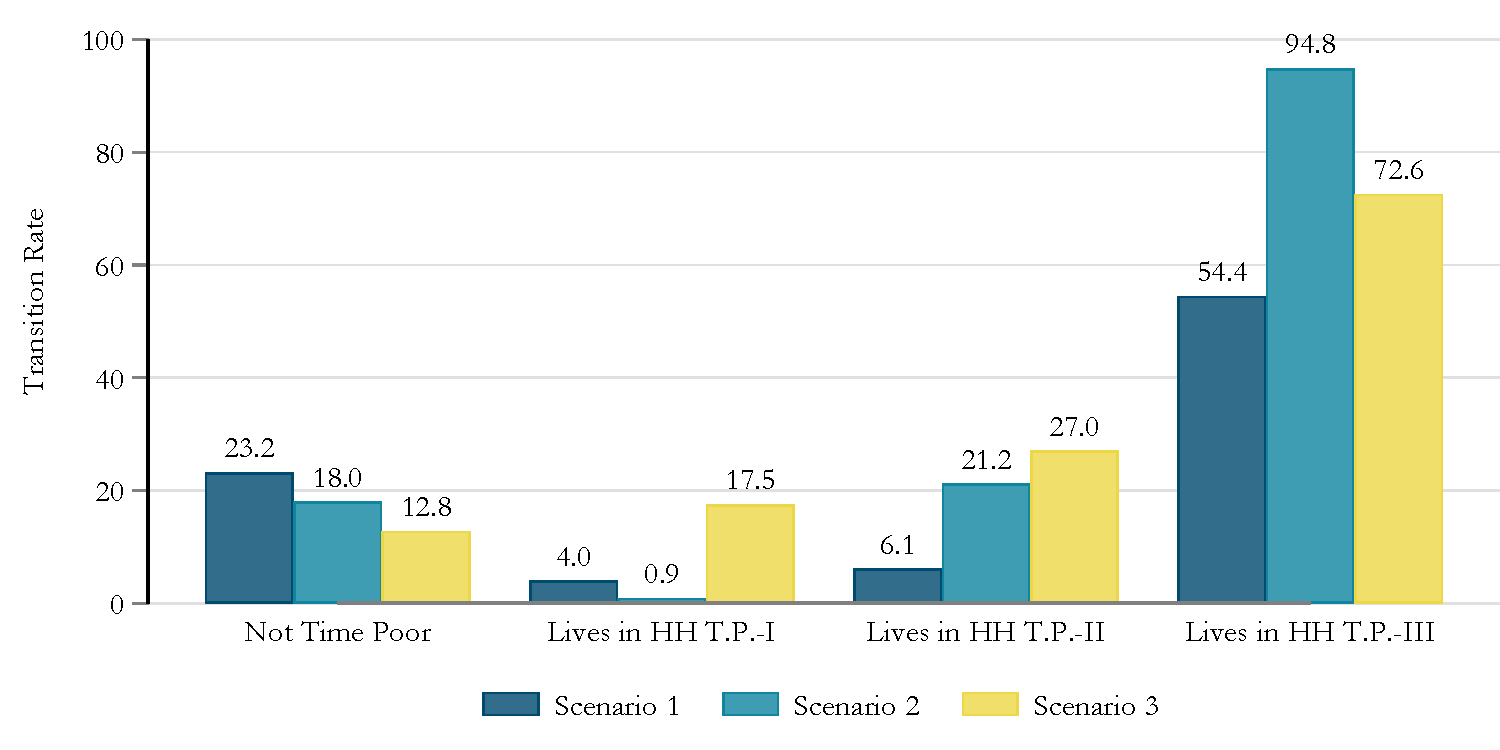
\includegraphics{resources_brief/poverty_men.pdf}

\footnotesize Note: The transition rates are calculated as the share of
individuals who change their time poverty status as a result of the
redistribution simulation.

}

\caption{\label{fig-transition1}Transition rates: Men in Couple}

\end{figure}%

The one that is more striking, however, is the redistribution based on
opportunity cost. It may seem that because men are more likely to have
higher wages, they are also less likely to take up more household
responsibilities compared to women. In consequence, while 12.8\% of
non-time poor men will fall into time poverty, 16.5\% of women will do
so under scenario 3.

The results for couples living in households type I and II are
strikingly similar. For men, if almost everyone in their household is
time-poor, preventing the household from escaping time poverty, their
transition rates out of poverty are small (4\% under Scenario 1 and 1\%
under Scenario 2). This is expected, as there is very little room for
redistribution. Interestingly, however, women's transition rates out of
time poverty are much higher (32.3\%) under scenario 1, and a small
1.5\% under scenario 2. In all three redistribution scenarios
women/wives are more likely than men to exit poverty, and while the
houshold would not be aboe to get out of poverty, there are likely some
gender-equitable redistribution outcomes.

Something unexpected was that under scenario 3, both men and women in
households type I and II show similar transition rates out of time
poverty, with only a slightly larger impact for men in household type
II. This is rather surprising because of the well-known wage gaps
between husbands and wives. Nevertheless, because this scenario favors
those with higher earning potential, working men and women benefit from
this scenario. The question that remains is whether this is a good
thing, or who within the household is taking up the extra
responsibilities.

The last group of interest are those living in households type III. As
described earlier, these are the only households where redistribution
could eliminate time poverty, and the different scenarios clearly show
that this is possible. As shown in Figure~\ref{fig-transition1} and
Figure~\ref{fig-transition2}, regardless of the scenario, at least 54\%
of men and 73\% of women exit time poverty as a result of
redistribution. In relative terms, women benefit the most compared to
men under the first scenario. Under Scenario 3, which favors those with
higher earning potential, the figures show similar transition rates for
men and women (73\%). However, the scenario that does the best in
reducing time poverty is the second one, which redistributes
responsibilities based on time availability. In this case, nearly every
couple (95\% men and 97\% women) is able to exit time poverty.

\begin{figure}[H]

\centering{

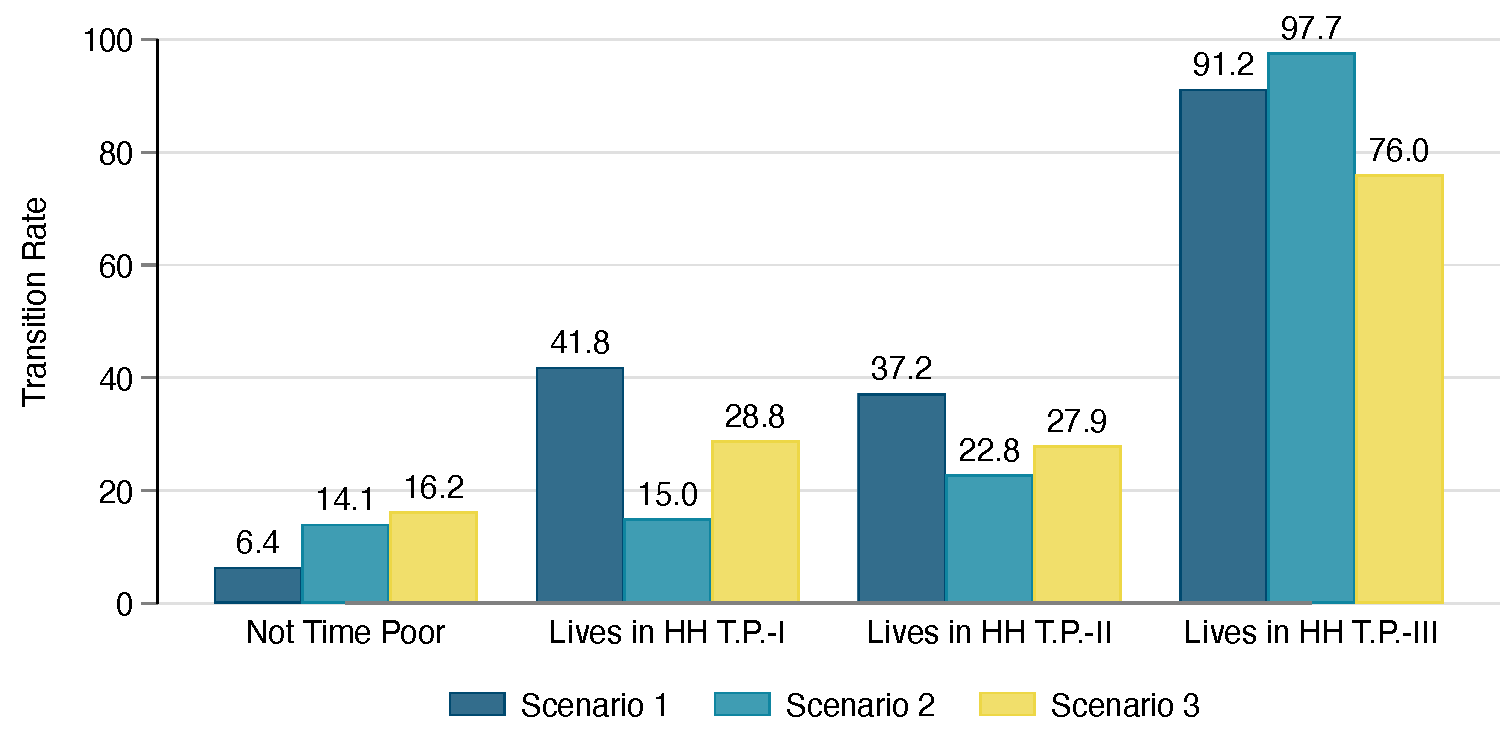
\includegraphics{resources_brief/poverty_wmen.pdf}

\footnotesize Note: The transition rates are calculated as the share of
individuals who change their time poverty status as a result of the
redistribution simulation.

}

\caption{\label{fig-transition2}Transition rates: Women in Couple}

\end{figure}%

Across all these scenarios, the remaining question is what is happening
with other household members. As shown in Table~\ref{tbl-class2}, other
individuals in the household have a similar or lower time poverty rate
compared to couples. And while they represent less than 8\% of the
population living in households type I and II, they represent 28\% of
the population in households type III, which makes them a relevant group
to consider. As shown in Figure~\ref{fig-transition3}, there is a small
proportion of non-time poor that fall into time poverty, with the
highest impact under Scenario 3 (7\%), still lower compared to couples
in the household. Among household type III, where they represent a
sizable share of the sample, their transition rates out of poverty are
just as high as for couples, but showing less variation across
scenarios. This suggests that the redistribution scenarios are also
effective in helping them exit time poverty, hinting at the possibility
that they are taking up some of the extra responsibilities without
pushing them into time poverty.

\begin{figure}[H]

\centering{

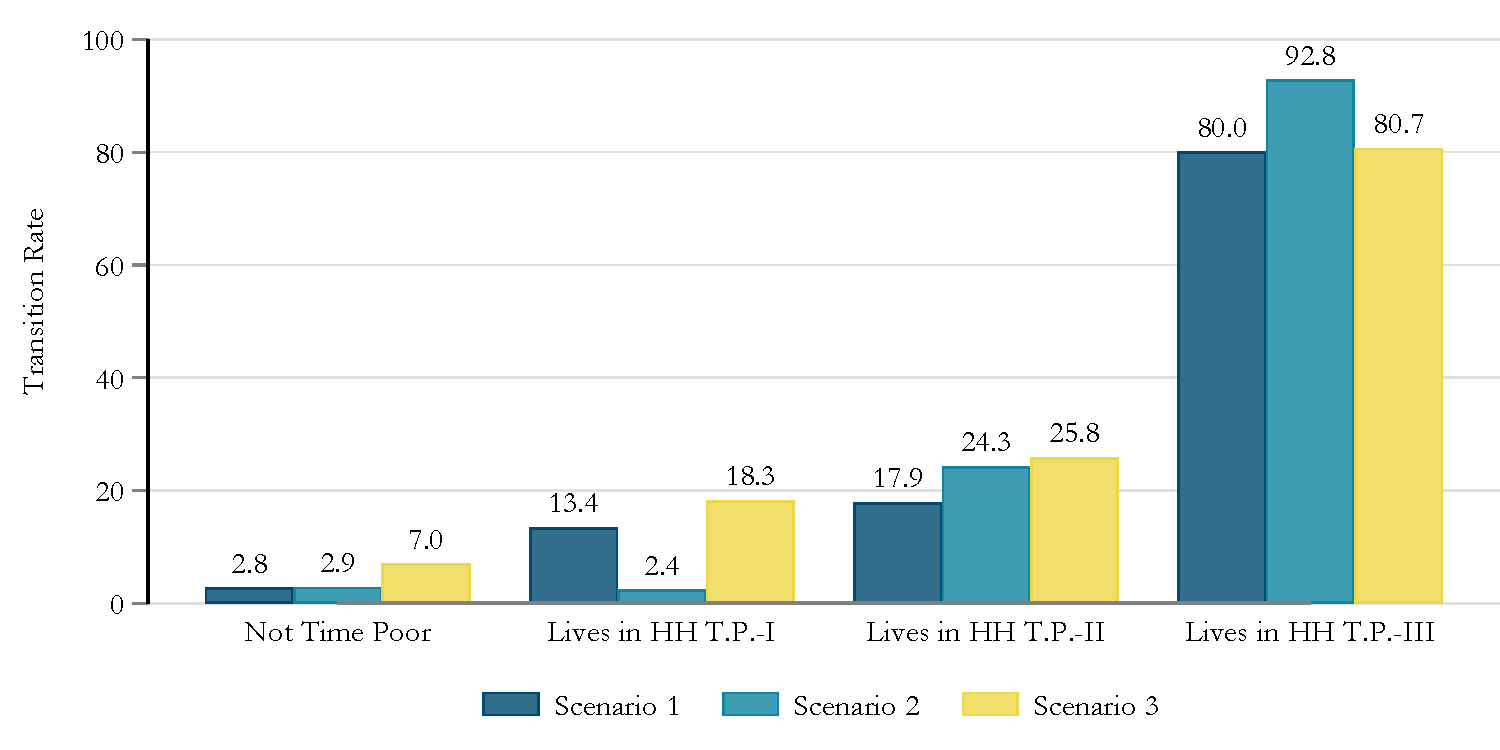
\includegraphics{resources_brief/poverty_other.pdf}

\footnotesize Note: The transition rates are calculated as the share of
individuals who change their time poverty status as a result of the
redistribution simulation.

}

\caption{\label{fig-transition3}Transition rates: Other Individuals (not
in a couple)}

\end{figure}%

\subsection{Redistribution Scenarios and Time
Deficits}\label{redistribution-scenarios-and-time-deficits}

The transition rates provide a good description of how redistribution
scenarios impact time poverty. However, they do not provide insights
into the magnitude of the changes in time deficits that individuals
face. In this section, we present the average time deficits individuals
face under different redistribution scenarios, focusing on the different
household types. To analyze the changes in time deficits, we provide
estimates for the average time deficits under different redistribution
scenarios, by group.

We start by considering the case of men that belong to a couple. On
average, after redistribution, non-time poor individuals will face a
time deficit of 0.7-1.4 hours per week, depending on the scenario. For
those who fall into time poverty, however, these changes imply an
average time deficit between 5 to 6 hours per week. This is still small
compared to the time deficits of individuals who start as time-poor. For
women, the average time deficit for non-time poor individuals is 0.2-1.0
hours, or 3.8-6.32 hours for those who fall into time poverty. While
falling into time poverty is not ideal, it is interesting to note that
men end up with a larger time deficit compared to their partners.

The case of those living in households type I is somewhat different.
Because there are people who are able to exit time poverty, their
responsibilities had to be redistributed among other household members.
Based on Figure~\ref{fig-def1}, under scenario 1, time-poor men would
take on more responsibilities, increasing their time deficit by just
under 6 hours a week. In the same scenario, women would see a reduction
in their time deficit of 4 hours, which would cause a type of reverse
gender gap. In other scenarios, changes are less dramatic, with only
marginal changes in time deficits.

For households type II, it is interesting to notice that those who are
time-poor face larger time deficits compared to people living in
households type I. The redistribution scenario 1 drastically favors
women, reducing their time deficit by 14 hours, although men would also
see a reduction of 7 hours in their time deficit. Scenarios 2 and 3
would have similar impacts reducing time deficits for men and women (15
hours and 10 hours respectively). Albeit scenario 3 was more effective
in reducing time poverty, compared to scenario 2 which fosters a more
equitable redistribution of responsibilities.

In households type III, both men and women (who were time-poor) have
similar time deficits before redistribution (about 10 hours per week).
However, after redistribution, the average time deficits among women
practically disappear, although reductions are less dramatic for men. In
both cases, the remarkable reduction in time deficits is explained by
the large poverty exit rates observed before. A simple transformation
suggests that, among men, those who remain time-poor still face a time
deficit of nearly 10 hours per week, except under scenario 2, where the
time deficit is reduced to 5.5 hours. For women who remain time-poor,
however, their time deficit is reduced by at least 3 hours per week
(Scenario 2) or up to 5 hours (Scenario 3).

\begin{figure}[H]

\centering{

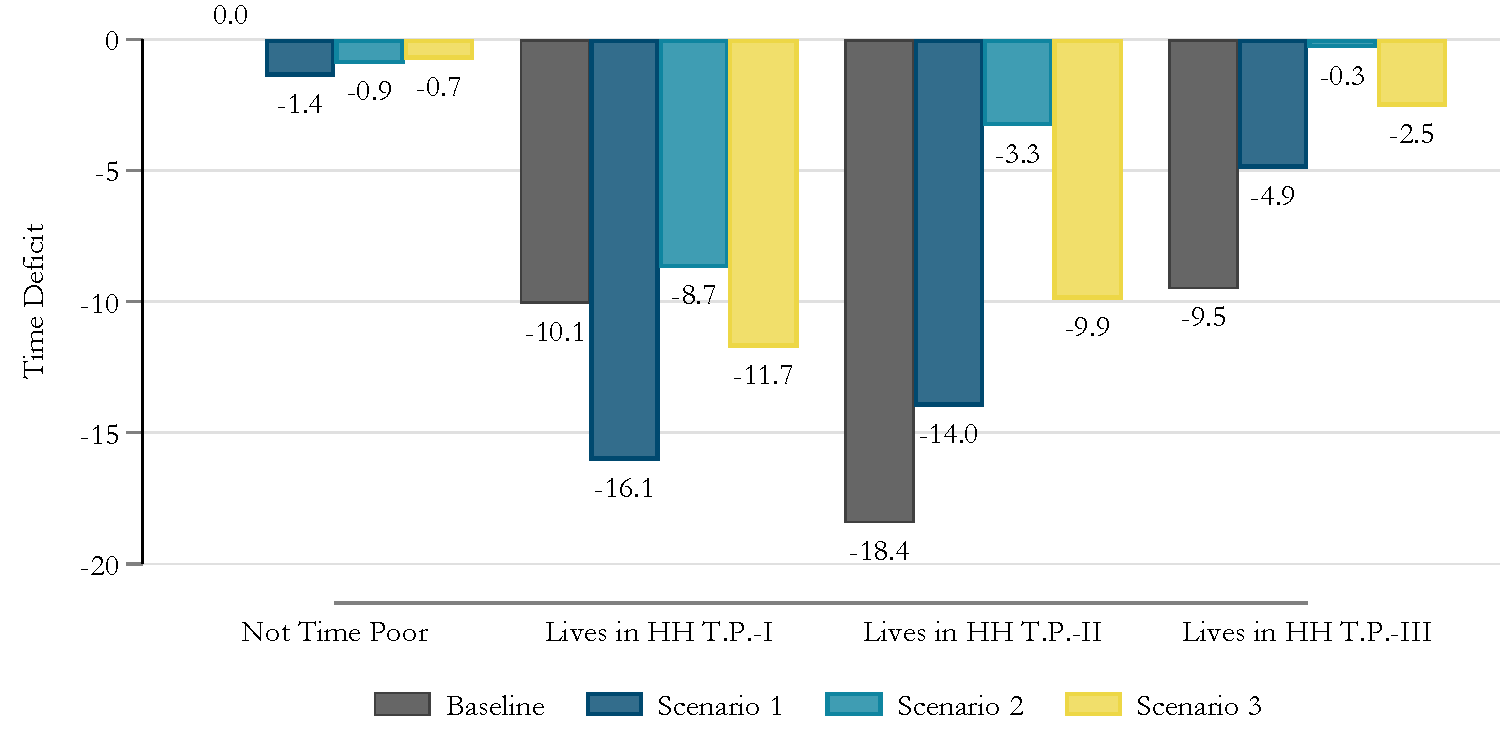
\includegraphics{resources_brief/tdef_men.pdf}

}

\caption{\label{fig-def1}Time Deficits by Individual type: Men}

\end{figure}%

\begin{figure}[H]

\centering{

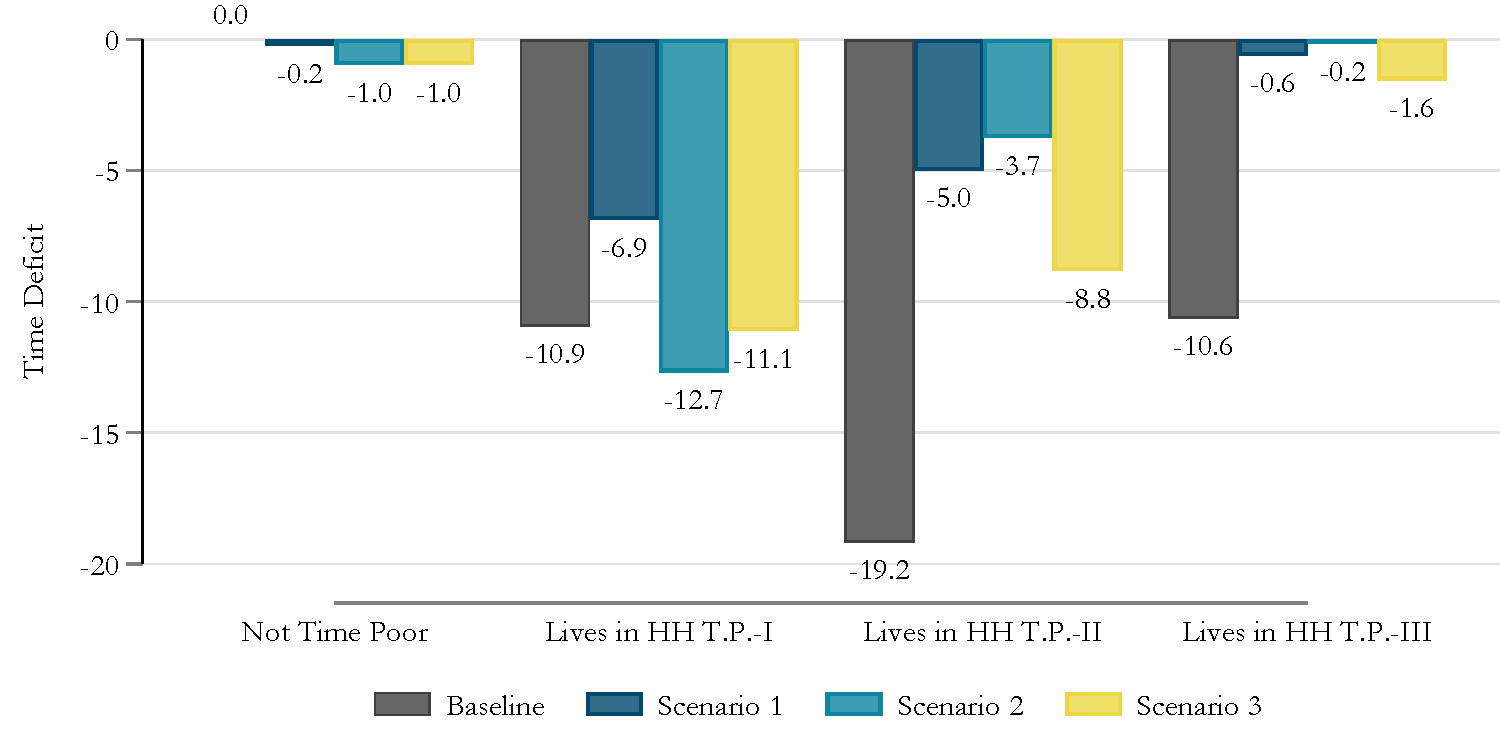
\includegraphics{resources_brief/tdef_wmen.pdf}

}

\caption{\label{fig-def2}Time Deficits by Individual type: Women}

\end{figure}%

There is, of course, the question of what happens for other members. As
shown in Figure~\ref{fig-def3}, the redistribution scenarios have, on
average, a small impact on those who were not time-poor before
redistribution. Although those who enter time poverty face deficits of
about 2-5 hours per week, depending on the scenario. This is still below
the time deficit time-poor people face before redistribution. In
contrast with couples, non-couple household members face almost no
change in their time deficits if they live in households type I. For
those living in households type II, scenario 2 (time available)
generates the largest benefits in terms of deficit reduction
(\textasciitilde14 hours), but they seem to be somewhat indifferent
between scenarios 1 and 3.

\begin{figure}[H]

\centering{

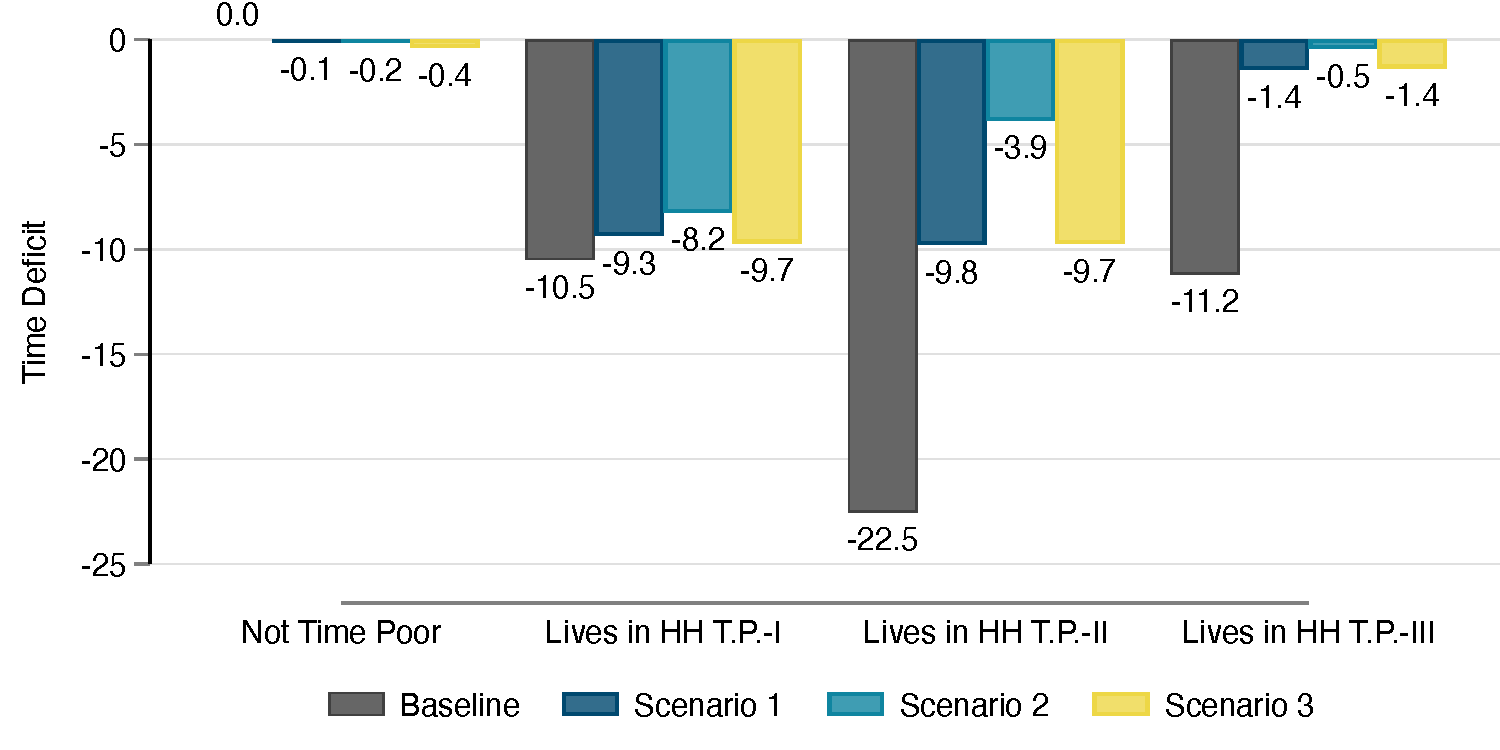
\includegraphics{resources_brief/tdef_other.pdf}

}

\caption{\label{fig-def3}Time Deficits by Individual type: Other
Individuals (not in a couple)}

\end{figure}%

\subsection{Changes in LIMTIP: The hidden
poor}\label{changes-in-limtip-the-hidden-poor}

While the discussion above provides a picture of the potential impact
that redistribution could have on time poverty, it is equally important
to understand changes in terms of Adjusted Poverty/LIMTIP estimates. In
other words, are the redistribution scenarios able to reduce the
incidence of hidden poor?

In this section, we provide some insights into how the redistribution
scenarios could impact the incidence of LIMTIP poverty among time-poor
households.

We first consider the household as a whole. As shown earlier, time-poor
households are the least affected by income poverty. Evidently, they
engage in a trade-off between time and income poverty, favoring work
over being non-time poor. As can be observed in
Figure~\ref{fig-limtip1}, only 4.1\% of individuals in time-poor
households are income poor, according to the official SPM poverty
line.\footnote{This estimate is different from Table~\ref{tbl-limtip}
  because Figure~\ref{fig-limtip1} does not include ``single''
  households.} However, given their time poverty status, the LIMTIP
estimates show that 9.2\% of individuals live in time-poor households,
which translates to 5.1\% of individuals being hidden poor.

When considering the different scenarios, despite the different nature
of the redistribution criteria, they all have considerably similar
effects on time poverty, reducing the incidence of hidden poor from 5\%
to only 1-2\% for all households combined, with Scenario 2 (time
availability) proving to be the most effective in reducing hidden
poverty. The decline in the incidence of hidden poor is the highest for
households Type II, about 4-5\%.

The only case where this does not happen is among households Type I.
Because everyone in this household is time-poor, redistribution is able
to reduce the incidence of time poverty at the individual level, at the
expense of sometimes increasing household time poverty, and hence LIMTIP
poverty. In addition, because of the limited room for redistribution,
households type II are only able to reduce hidden poverty by half,
whereas in households type III, the hidden poor are practically
eliminated (0.2-0.6\%).

\begin{figure}[H]

\centering{

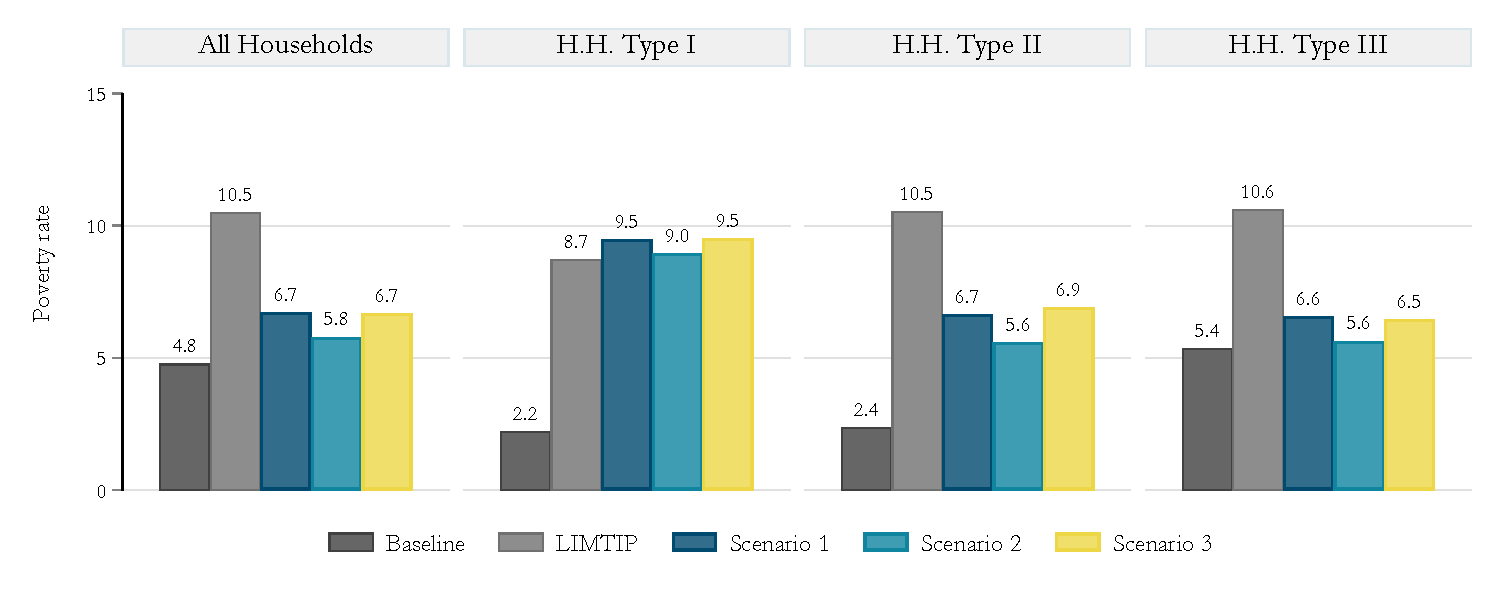
\includegraphics{resources_brief//hh_pov.pdf}

}

\caption{\label{fig-limtip1}Changes in Poverty estimates across
redistribution scenarios: Household}

\end{figure}%

\section{Policy implications}\label{policy-implications}

The findings in this policy brief suggest that intra-household
redistribution of household production is a potentially effective tool
to reduce time deficits and alleviate time poverty for individuals and
households. Our findings show that such redistributions can have
significant well-being effects, promoting more equitable sharing of
household responsibilities between men and women and, in some cases,
lifting entire households out of poverty.

However, the effectiveness of redistribution policies is contingent on
the context of each household. For instance, in households where all
members are time-poor, redistribution may not be effective and could
potentially (slightly) increase LIMTIP poverty. In contrast, households
with sufficient time surpluses to absorb time deficits can effectively
eliminate time poverty under any of the proposed redistribution
policies.

Among the three redistribution scenarios considered, the equity-based
approach emerged as the most effective in reducing poverty rates and
enabling individuals to exit poverty.

While the study examined redistribution among all working-age members
(18-64 years), future research and policy development should consider
more targeted approaches. Specifically, focusing on redistribution
between men and women within specific age groups, or with or without
children, could provide better information to propose policies that
avoid potential negative impacts of penalizing younger or older
household members by redistributing household burden to members of these
age groups. This as evidence supports may prove to be detrimental and
have vicous cycle effects if the penalizing is particulalry restricted
to younger girls {[}will elaborate and add citations{]}.

Future work should consider analyzing the composition of household
production, in addition to redistribution. This would allow for the
elaboration of more detailed public policies that consider the specific
needs of households such as provision of childcare, eldercare, or other
services that could help reduce household production requirements and
time deficits.

\section{Conclusion}\label{conclusion}

This policy brief has examined the potential of redistributing household
production responsibilities to alleviate time poverty in the United
States. Using the Levy Institute Measure of Time and Income Poverty
(LIMTIP), we have shown that time poverty is a significant issue
affecting 38.7\% of individuals living in time-poor households. Our
analysis of three redistribution scenarios - based on equality, equity,
and opportunity cost principles - reveals that such redistributions can
significantly reduce time poverty, particularly in households where time
surpluses exceed time deficits.

These findings underscore the importance of considering time poverty in
poverty alleviation efforts. They also highlight the potential of
intra-household redistribution as a policy tool to promote gender
equality and improve overall household well-being. However, the varying
effects across household types and scenarios suggest that a
one-size-fits-all approach may not be optimal, and that further research
on this area is needed.

In conclusion, while redistribution of household production is promising
in alleviating time poverty, and the hidden poor, it should be
considered as part of strategies that also addresses societal and
structural factors that contribute to time and income poverty.

\section*{References}\label{sec-ref}
\addcontentsline{toc}{section}{References}

\phantomsection\label{refs}
\begin{CSLReferences}{1}{0}
\bibitem[\citeproctext]{ref-addati2018}
Addati, L., Cattaneo, U., Esquivel, V., and Valarino, I. (2018).
\emph{Care work and care jobs for the future of decent work}.
International Labour Organisation (ILO).

\bibitem[\citeproctext]{ref-Antonopoulos2017}
Antonopoulos, R., Esquivel, V., Masterson, T., and Zacharias, A. (2017).
Time and income poverty in the city of buenos aires. In R. Connelly and
E. Kongar (Eds.), \emph{Gender and time use in a global context: The
economics of employment and unpaid labor} (pp. 161--192). Palgrave
Macmillan US. \url{https://doi.org/10.1057/978-1-137-56837-3_7}

\bibitem[\citeproctext]{ref-berik2009}
Berik, G., Rodgers, Y. van der M., and Seguino, S. (2009). Feminist
{Economics} of {Inequality}, {Development}, and {Growth}. \emph{Feminist
Economics}, \emph{15}(3), 1--33.
\url{https://ezprox.bard.edu/login?url=https://search.ebscohost.com/login.aspx?direct=true&db=ecn&AN=1063369&site=eds-live&scope=site}

\bibitem[\citeproctext]{ref-hundt1996}
Bruyn-Hundt, M. (1996). Scenarios for a redistribution of unpaid work in
the netherlands. \emph{Feminist Economics}, \emph{2}(3), 129--133.
\url{https://doi.org/10.1080/13545709610001707826}

\bibitem[\citeproctext]{ref-duflo2012}
Duflo, E. (2012). Women {Empowerment} and {Economic} {Development}.
\emph{Journal of Economic Literature}, \emph{50}(4), 1051--1079.
\url{https://doi.org/10.1257/jel.50.4.1051}

\bibitem[\citeproctext]{ref-elson2017}
Elso, D. (2017). \emph{Recognize, {Reduce}, and {Redistribute} {Unpaid}
{Care} {Work}: {How} to {Close} the {Gender} {Gap}}.
\url{https://doi.org/10.1177/1095796017700135}

\bibitem[\citeproctext]{ref-elson2009}
Elson, D. (2009). Gender {Equality} and {Economic} {Growth} in the
{World} {Bank} {World} {Development} {Report} 2006. \emph{Feminist
Economics}, \emph{15}(3), 35--59.
\url{https://doi.org/10.1080/13545700902964303}

\bibitem[\citeproctext]{ref-valeria2016}
Esquivel, V. (2016). Power and the {Sustainable} {Development} {Goals}:
A feminist analysis. \emph{Gender \& Development}, \emph{24}(1), 9--23.
\url{https://doi.org/10.1080/13552074.2016.1147872}

\bibitem[\citeproctext]{ref-heckman1979}
Heckman, J. J. (1979). Sample selection bias as a specification error.
\emph{Econometrica}, \emph{47}(1), 153.
\url{https://doi.org/10.2307/1912352}

\bibitem[\citeproctext]{ref-hess2020}
Hess, Cynthia, Ahmed, T., and Hayes, J. (2020). \emph{Providing {Unpaid}
{Household} and {Care} {Work} in the {United} {States}: {Uncovering}
{Inequality}}.

\bibitem[\citeproctext]{ref-malik2018}
Malik, R., Hamm, K., Schochet, L., Novoa, C., Workman, S., and
Jessen-Howard, S. (2018). America's {Child} {Care} {Deserts} in 2018.
\emph{Center for American Progress}.
\url{https://www.americanprogress.org/article/americas-child-care-deserts-2018/}

\bibitem[\citeproctext]{ref-masterson2012}
Masterson, T. (2012). \emph{Simulations of full-time employment and
household work in the levy institute measure of time and income poverty
(LIMTIP) for argentina, chile, and mexico} (Working Paper 727; Levy
Economics Institute Working Paper). Levy Economics Institute of Bard
College.

\bibitem[\citeproctext]{ref-masterspm2022}
Masterson, T., Antonopoulos, R., Nassif-Pires, L., Rios-Avila, F., and
Zacharias, A. (2022). \emph{Assessing the impact of childcare expansion
in mexico: Time use, employment, and poverty} {[}Research Project
Report{]}. Levy Economics Institute of Bard College.
\url{https://www.levyinstitute.org/pubs/rpr_6_22.pdf}

\bibitem[\citeproctext]{ref-oecd2020}
OECD. (2020). \emph{Early learning and child well-being in the united
states} (p. 124).
https://doi.org/\url{https://doi.org/https://doi.org/10.1787/198d8c99-en}

\bibitem[\citeproctext]{ref-rein2023}
Reinhard, S. C., Caldera, S., Houser, A., and Choula, R. (2023).
\emph{Valuing the {Invaluable}: 2023 {Update}}. AARP Public Policy
Institute. \url{https://doi.org/10.26419/ppi.00082.006}

\bibitem[\citeproctext]{ref-zacharias2011}
Zacharias, A. (2011). \emph{The measurement of time and income poverty}
(Working Paper 690; Levy Economics Institute Working Paper). Levy
Economics Institute of Bard College.

\bibitem[\citeproctext]{ref-zacharias2012}
Zacharias, A., Antonopoulos, R., and Masterson, T. (2012). \emph{Why
time deficits matter: Implications for the measurement of poverty}
{[}Research Project Report{]}. Levy Economics Institute of Bard College.
\url{https://www.levyinstitute.org/pubs/rpr_08_12}

\bibitem[\citeproctext]{ref-zacharias2014}
Zacharias, A., Masterson, T., and Kim, K. (2014). \emph{The measurement
of time and income poverty in korea: The levy institute measure of time
and income poverty} {[}Research Project Report{]}. Levy Economics
Institute of Bard College.
\url{https://www.levyinstitute.org/pubs/rpr_8_14}

\bibitem[\citeproctext]{ref-zacharias2018}
Zacharias, A., Masterson, T., Rios-Avila, F., Kim, K., and
Khitarishvili, T. (2018). \emph{The measurement of time and income
poverty in ghana and tanzania: The levy institute measure of time and
consumption poverty} {[}Research Project Report{]}. Levy Economics
Institute of Bard College.
\url{https://www.levyinstitute.org/pubs/rpr_8_18}

\bibitem[\citeproctext]{ref-zacharias2021}
Zacharias, A., Masterson, T., Rios-Avila, F., and Oduro, A. D. (2021).
\emph{Scope and effects of reducing time deficits via intrahousehold
redistribution of household production: Evidence from sub-saharan
africa: The levy institute measure of time and consumption poverty}
{[}Research Project Report{]}. Levy Economics Institute of Bard
College.\href{\%20https://www.levyinstitute.org/pubs/rpr_7_21.pdf}{https://www.levyinstitute.org/pubs/rpr\_7\_21.pdf}

\bibitem[\citeproctext]{ref-zacharias2024a}
Zacharias, A., Rios-Avila, F., Folbre, N., and Masterson, T. (2024).
\emph{Integrating nonmarket consumption into the bureau of labor
statistics consumer expenditure survey} {[}Research Project Report{]}.
Levy Economics Institute of Bard
College.\href{\%20https://www.bls.gov/cex/consumption/integrating-nonmarket-consumption-bls-consumer-expenditure-survey.pdf}{https://www.bls.gov/cex/consumption/integrating-nonmarket-consumption-bls-consumer-expenditure-survey.pdf}

\end{CSLReferences}



\end{document}
